\documentclass[11pt]{article}

% Document settings, taken from Introduction to Algorithms (Dinitz).
\usepackage{epsfig}
\usepackage{amsfonts}
\usepackage{amssymb}
\usepackage{amstext}
\usepackage{amsmath}
\usepackage{xspace}
\usepackage{hyperref}
\usepackage{fullpage}
\usepackage{enumitem}                     
\usepackage{titlesec}
\usepackage{amsthm}
\usepackage{natbib}

\hypersetup{
    colorlinks=true,
    linkcolor=blue,
    filecolor=magenta,      
    urlcolor=cyan,
}

\titleformat*{\section}{\bfseries}
\titleformat*{\subsection}{\bfseries}
\titleformat*{\subsubsection}{\bfseries}
\titleformat*{\paragraph}{\bfseries}
\titleformat*{\subparagraph}{\bfseries}

\newcommand{\R}{\ensuremath{\mathbb R}}
\newcommand{\C}{\ensuremath{\mathbb C}}
\newcommand{\N}{\ensuremath{\mathbb N}}
\newcommand{\F}{\ensuremath{\mathbb F}}
\newcommand{\K}{\ensuremath{\mathbb K}}
\newcommand{\Z}{\ensuremath{\mathbb Z}}
\newcommand{\B}{\ensuremath{\mathcal B}}
\renewcommand{\H}{\ensuremath{\mathcal H}}
\newcommand{\EV}{\ensuremath{\mathbb E}}
\newcommand{\Var}{\text{Var}}
\newcommand{\Cov}{\text{Cov}}
\newcommand{\e}{\epsilon}
\newcommand{\E}{\exists}
\newcommand{\sse}{\subseteq}
\newcommand{\union}{\cup}
\newcommand{\ra}{\rightarrow}
\newcommand{\ceil}[1]{\ensuremath{\left\lceil#1\right\rceil}}
\newcommand{\floor}[1]{\ensuremath{\left\lfloor#1\right\rfloor}}
\newcommand{\ip}[2]{\left\langle #1, #2\right\rangle}
\DeclareMathOperator*{\argmax}{arg\,max\ }
\DeclareMathOperator*{\argmin}{arg\,min\ }

\theoremstyle{plain}
\newtheorem{thm}{Theorem}[section]
\newtheorem{lem}{Lemma}[section]
\newtheorem{prop}{Proposition}[section]
\newtheorem{coro}{Corollary}[section]
\newtheorem{obs}{Observation}[section]

\theoremstyle{definition}
\newtheorem{defi}{Definition}[section]

\theoremstyle{remark}
\newtheorem{exm}{Example}[section]
\newtheorem{exc}{Exercise}[section]
\newtheorem{rem}{Remark}[section]
\newtheorem{question}{Question}
\newtheorem{answer}{Answer}

\setenumerate[0]{label=(\alph*)}


%%%%%%%%%%%%%%%%%%%%%%%%%%%%%%%%%%%%%%%%%%%%%%%%%%%%%%%%%%%%%%%%%%%%%%%%%%%
%%%%%%%%%%%%%%%%%%%%%%%%%% Document begins here %%%%%%%%%%%%%%%%%%%%%%%%%%%
%%%%%%%%%%%%%%%%%%%%%%%%%%%%%%%%%%%%%%%%%%%%%%%%%%%%%%%%%%%%%%%%%%%%%%%%%%%


\begin{document}

% EDIT THE FOLLOWING PARAMETERS FOR EACH ASSIGNMENT.

% NAME and COURSE TITLE + SECTION NUMBER
\noindent {\large {\bf Mathematical Thinking and Proof-Writing for Engineers}} \hfill {\bf Intersession 2020}

% PROFESSOR and HOMEWORK NUMBER
\noindent {{\bf Instructor:} Ronak Mehta} \hfill 
{Class Notes}

\noindent \rule[0.1in]{\textwidth}{0.4pt}

% CONTENT

\section{January 6, 2020}

\paragraph{Prereading} \href{https://drive.google.com/drive/folders/1T_M-dvYE4leOSmpKt2eGYOvPRch_SDpK?usp=sharing}{Pages 1 - 11} of {\it Mathematics: A Discrete Introduction} by Edward Scheinerman.

\subsection{Introduction}
Welcome, and thanks for your interest! While mathematical theory is usually not the poster boy of engaging and topical intersession courses, I think we can change some minds with this particular class. The subject is fascinating, but notoriously difficult to teach. There are many balancing acts when it comes to mathematical education; those of memorization versus exploration, theory versus application, and lectures versus self-guided learning constitute most of the battle. In any case, I can make a strong argument for the utility of this course in your future endeavors, so I'll attempt to present it in a way that is best for you. To this end, I ask of you all a healthy amount of honest and constructive feedback throughout the course.

As a brief introduction, I recently graduated from the Master's program in Applied Mathematics and Statistics at Hopkins in May. Generally, I have focused my education around the mathematical foundations of data science - namely statistics, linear algebra, and optimization. I currently work in the \href{https://neurodata.io/}{lab of Dr. Joshua Vogelstein} in the Department of Biomedical Engineering, where I develop statistical procedures for neuroimaging data. I've also recently gone through a round of Ph.D. applications in data science, so hopefully you will hear some good news over the course of this class!

First, let us motivate this class, both in a general sense, and a way that applies to you directly. The most recent \href{https://hechingerreport.org/what-2018-pisa-international-rankings-tell-us-about-u-s-schools/}{Programme for International Student Assessment (PISA)} in 2018 ranked the U.S. at 36th out of 79 countries in mathematics. For decades, American math proficiency has compared abysmally to other developed nations, and since the 1980's the ``\href{https://en.wikipedia.org/wiki/Math_wars}{math wars}" debate pits rote memorization versus inquiry-based approaches to learning. I am personally unconvinced that such a dichotomy exists, given how many American debates typically present only two, fundamentally opposing options against one another. Moreover, these kinds of assessments come from a place of ``\href{http://neatoday.org/2019/12/03/2018-pisa-results/}{mental Olympics}" competitions for countries, as well as a measure of how prepared students are for a modern job market.  While this is a fine perspective, also consider the beauty and virtue that mathematics holds in and of itself. 

Paul Lockhart, in his book {\it A Mathematician's Lament}, compares current mathematics education to a dystopian version of teaching music.\\
\setlength{\leftskip}{1cm}

Since musicians are known to set down their ideas in the form of sheet music, these curious black dots and lines must constitute the ``language of music.” It is imperative that students become fluent in this language if they are to attain any degree of musical competence; indeed, it would be ludicrous to expect a child to sing a song or play an instrument without having a thorough grounding in music notation and theory. Playing and listening to music, let alone composing an original piece, are considered very advanced topics and are generally put off until college, and more often graduate school...

In the higher grades the pressure is really on. After all, the students must be prepared for the standardized tests and college admissions exams. Students must take courses in Scales and Modes, Meter, Harmony, and Counterpoint. ``It’s a lot for them to learn, but later in college when they finally get to hear all this stuff, they’ll really appreciate all the work they did in high school.” Of course, not many students actually go on to concentrate in music, so only a few will ever get to hear the sounds that the black dots represent. Nevertheless, it is important that every member of society be able to recognize a modulation or a fugal passage, regardless of the fact that they will never hear one. ``To tell you the truth, most students just aren’t very good at music. They are bored in class, their skills are terrible, and their homework is barely legible. Most of them couldn’t care less about how important music is in today’s world; they just want to take the minimum number of music courses and be done with it. I guess there are just music people and non-music people. I had this one kid, though, man was she sensational! Her sheets were impeccable— every note in the right place, perfect calligraphy, sharps, flats, just beautiful. She’s going to make one hell of a musician someday.”\\

\setlength{\leftskip}{0pt}

Proof-writing is the fabric of true mathematics, where we put aside canned procedures and dig into our creativity. In fact, to my knowledge, math is the only arena where participants can truly discuss ideas with pure, irrefutable logic. Other settings, such as courtrooms and debate clubs may come close, but there is always an element of qualification, uncertainty, or human emotion in the mix. It is entirely possible to just have fun with mathematics, and our education system should reflect that. (What are your thoughts?)

Bringing the discussion back to home base, you all will take one of either automata, algorithms, kinematics, signal processing, or even graduate AMS courses in the near future. Being successful in these settings will rely on a deep mathematical foundation. Ren\'e Vidal (data science professor in the BME department) often tells his advisees that there is a moment where these previously disparate concepts really click, and learning math becomes easy and natural. My goal is that this happens for each of you during this course. We will be experimenting in two ways. First, we will shy away from the dichotomy of memorization and experimentation. Instead, while there are certain definitions I will ask you to memorize and have available for rapid recall, I will also observe and refine the way you tackle new problems. I hope that as a result, you achieve a flexible, enduring problem-solving approach. Second, class meetings will include both example problems that I will do, and exercise problems that you will do. As of now, I do not plan to have required homework besides some readings but will give you plenty of practice problems to work through together as the class goes on.

The class will include topics from Chapter 1 and 2 of {\it Mathematics: A Discrete Introduction} by Ed Scheinerman and most of {\it A Problem Book in Real Analysis} by Aksoy and Khamsi, which you can find \href{https://drive.google.com/drive/folders/1T_M-dvYE4leOSmpKt2eGYOvPRch_SDpK?usp=sharing}{here}. I really like both of them, especially due to their concision and clarity. Real analysis  is a course typically taken by math majors in their sophomore years. Some describe it as “Calc I done right”, in the sense of introducing similar topics but proving and deriving every result along the way. While there are many ways to practice proof-writing, I chose this particular content as to directly apply to graduate applied math courses, and practice heavily without introducing too much material. This includes proof strategies, sequences and series, limits, continuity, and point-set topology. We can add more content that is interesting to you as time permits. We will start off slow and basic, but things will ramp up quickly. Enjoy!

\subsection{Notation}

Descriptive and consistent notation supports understanding, so I will harp on notation (and terminology) slightly as we work through certain topics. However, we will do so as new topics are introduced, rather than all at once. If it is a helpful analogy, consider nomenclature in an organic chemistry class.

\subsection{Definitions, Theorems, Proofs}

% Before we get into the real nature of the course, we'll start with some visual examples to describe the kind of reasoning I we all develop. At some point in elementary school, you were told to accept that the circumference of a circle $C = 2\pi R$ where $R$ is the radius. This we can believe was discovered by measurement. However, we are also told that the area of a circle $A = \pi R^2$, volume of a sphere $V = \frac{4}{3} \pi R^3$, and the surface area of a sphere $S = 4 \pi R^2$. Let's start with something simpler, the area of a triangle $A_T = \frac{1}{2}bh$, where $b$ is the length of the base, and $h$ is the height.figure \ref{triangle} shows that splitting a scalene triangle into two right triangles makes clear why the formula holds. Letting the left base be $b_1$ and the right base be $b_2$, and noting that the right triangle's area is half that of the rectangle in which it is contained, we have
% \begin{align*}
%     A_T &= \frac{1}{2}b_1h + \frac{1}{2}b_2h\\
%     &= \frac{1}{2}(b_1 + b_2)h\\
%     &= \frac{1}{2}bh
% \end{align*}
% \begin{figure}
%     \centering
%     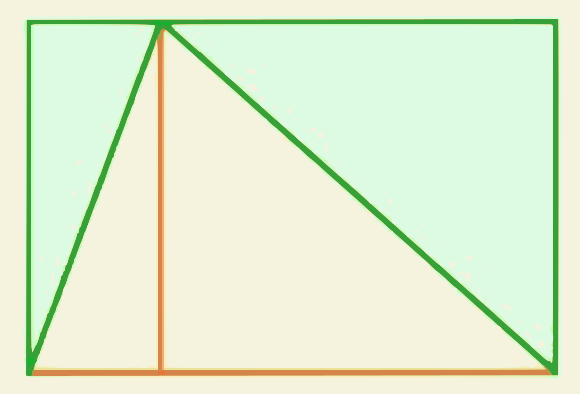
\includegraphics[width=0.6\linewidth]{figures/triangle.png}
%     \caption{We are interested in the area of the orange triangle, which has been split into two.}
%     \label{triangle}
% \end{figure}
% Similarly, we have the celebrated Pythagorean theorem, another formula we have been told to believe. Let $a$ and $b$ be two legs of a right triangle, and $c$ the hypotenuse. We know that $a^2 +b^2 = c^2$. How can we prove this? Take a look at Figure \ref{pyt}, and compute the area of 4 of these right triangles, both individually and by constructing a large square and subtracting the area of the square in the middle.
% \begin{figure}
%     \centering
%     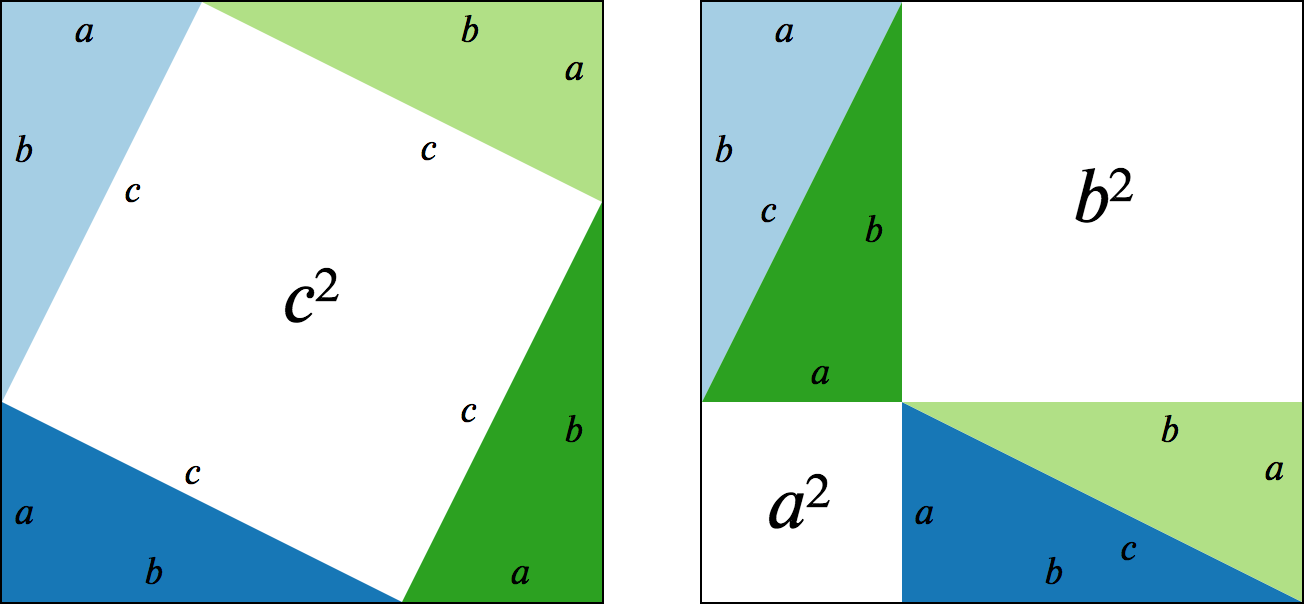
\includegraphics[width=0.6\linewidth]{figures/pythagorean.png}
%     \caption{Compute the area of the colored region both ways to prove the theorem.}
%     \label{pyt}
% \end{figure}
% \begin{align*}
%     4 \frac{1}{2} ab &= (a + b)^2 - c^2\\
%     2ab &= a^2 + 2ab + b^2 - c^2\\
%     c^2 &= a^2 + b^2
% \end{align*}

% Let's get back to the area of a circle. One of the most commonly known proofs is from about two thousand years ago by Archimedes (260 B.C.E.). For an $n$ side regular polygon , its area is going to be $A_n = \frac{1}{2} p_n a_n$, where $p_n$ is the perimeter and $a_n$ is the apothem (distance from center to midpoint of one of the sides). See \href{https://en.wikipedia.org/wiki/Area_of_a_circle#Archimedes's_proof}{Wikipedia} for the full proof. As in Figure \ref{circle}, the inscribed polygon will have perimeter approaching $2\pi R$, and apothem approaching $R$, as $n \rightarrow \infty$. The inscribed polygon also has less area than the circle. Letting $A$ be the area of the circle, we have
% \begin{align*}
%     A \geq \frac{1}{2} p_n a_n
% \end{align*}
% Taking the limit of both sides as $n$ gets large, we have
% \begin{align*}
%     A \geq \frac{1}{2} 2 \pi R \cdot R = \pi R^2
% \end{align*}
% For the circumscribed polygon, the apothem is always $R$, and the perimeter also approaches $2\pi R$. Thus,
% \begin{align*}
%     A \leq \frac{1}{2} p_n a_n = \frac{1}{2} p_n R
% \end{align*}
% Taking the limit once again, we have
% \begin{align*}
%     A \leq \frac{1}{2} 2 \pi &R \cdot R = \pi R^2\\
%     \implies \pi R^2 &\leq A \leq \pi R^2
% \end{align*}
% proving the area formula.

% \begin{figure}
%     \centering
%     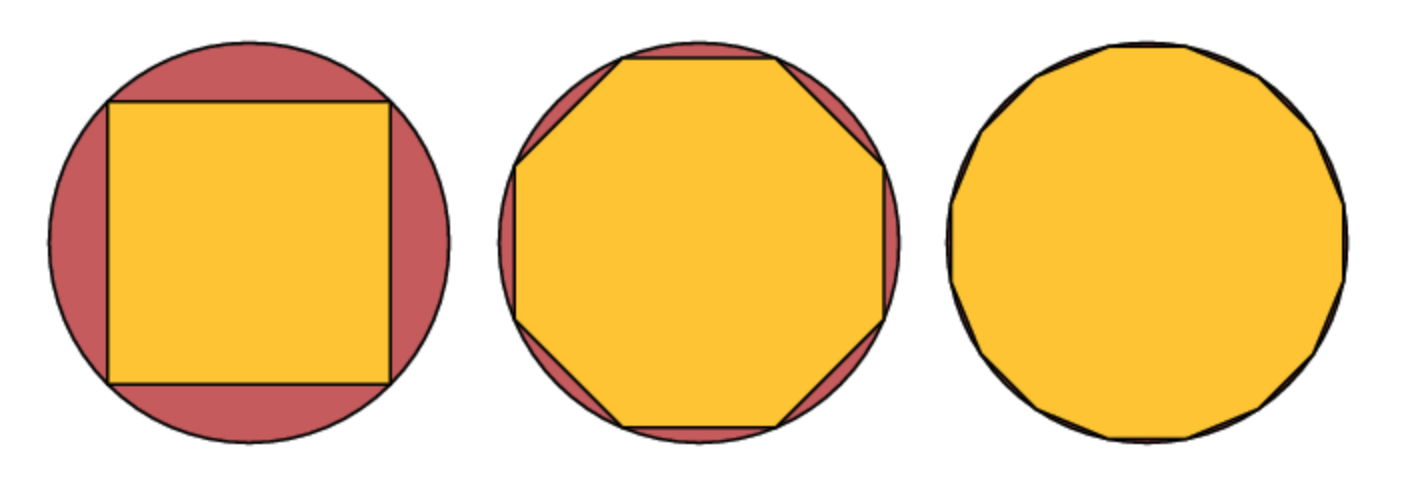
\includegraphics[width=0.6\linewidth]{figures/inscribed.png}
%     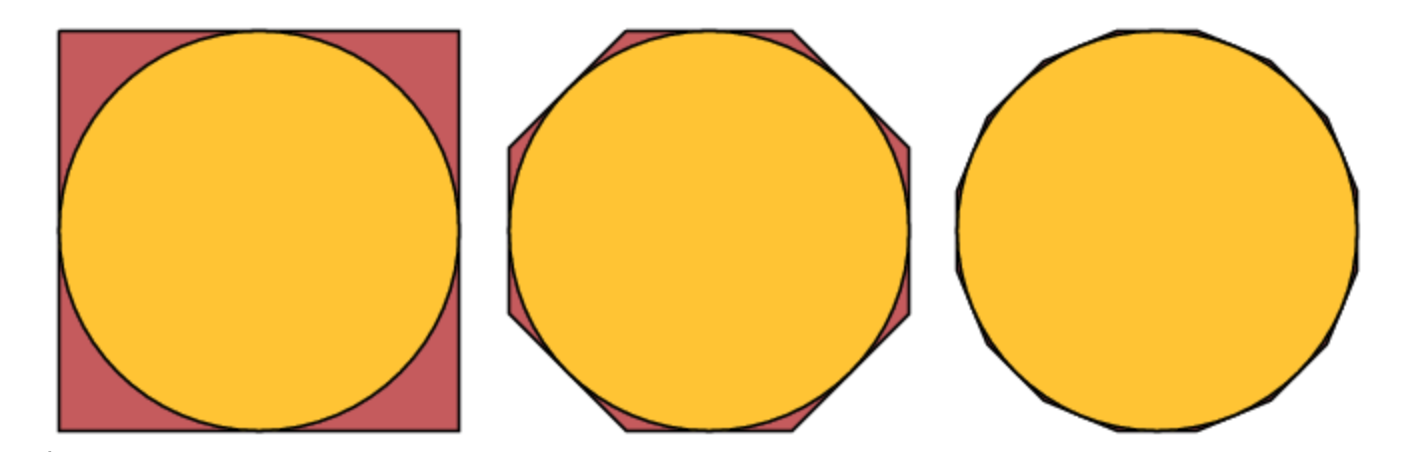
\includegraphics[width=0.6\linewidth]{figures/circumscribed.png}
%     \caption{The first panel shows an inscribed polygon, while the second shows the circumscribed polygon. Both approach the circle in area.}
%     \label{circle}
% \end{figure}


{\it Informal picture ``proofs" of area of triangle, Pythagorean theorem, area of a circle, volume of a sphere, and surface area of a sphere.}\\

Ed Scheinerman, currently the dean of our engineering school, can set the stage for you much better than I can. I especially like the first ten pages. Assuming that you've read through the chapter, you have come across definitions, theorems, and some basic proofs. We will not define ``definition" but take it as an introduction or a name of a mathematical object. In future classes, these should always be memorized and be able to be retrieved from your brain upon request. In order to understand, you must first memorize a little bit. On the other hand, theorems are declaritive statements which can be written of the form ``If [assumptions], then [conclusion]". More on this later.

\begin{defi}[Set]
    A set is a collection of unordered, distinct objects. 
\end{defi}
Sets can have a finite or infinite number of elements, and are usually denoted by capital letters. We can list their elements out one-by-one and wrap then in curly braces, or specify them by some condition, as in $\{x : \text{ condition regarding $x$ is true.}\}$. For example, 
\begin{align*}
    A = \{1, 2, 3, 6, 7\}
\end{align*}
is a set of 5 elements. Letting $\Z = \{..., -1, 0, 1, ...\}$ be the set of all integers, I can denote the same set by
\begin{align*}
    A = \{x \in \Z: 0 < x < 4 \text{ and } 5 < x < 8\}
\end{align*}
The colon within the braces can be read as ``such that". Let $\N = \{0, 1, 2, ...\} = \{x \in \Z: x \geq 0\}$ be the set of natural numbers, or nonnegative integers. Let's recall some definitions from the chapter.
\begin{defi}[Divisible]
    An integer $b$ is divides integer $a$ (written $b \mid a$) if there is an integer $c$ such that $a = bc$. $a$ is called a multiple of $b$, and is also called divisible by $b$. $b$ is also called a divisor or factor of $a$. 
\end{defi}
\begin{defi}[Even]
    An integer $a$ is called even if it is divisible by 2.
\end{defi}
\begin{defi}[Odd]
    An integer $a$ is called odd if there is an integer $x$ such that $a = 2x + 1$.
\end{defi}
\begin{defi}[Prime]
    An integer $p$ is called prime if $p > 1$ and the only positive divisors of $p$ are 1 and $p$.
\end{defi}
\begin{defi}[Composite]
    An integer $c$ is called composite if $c > 1$ and $c$ is not prime. We can also say integer $c > 1$ is composite if there exists a factor $b$ such that $1 < b < c$.
\end{defi}

While none of these concepts are particularly interesting in their own right, they are probably familiar to you. More importantly, with just these definitions, we have a huge class of problems with which to jump in and warm up. 

\begin{exc}
    Prove that the sum of two even integers is even.
\end{exc}
\begin{exc}
    Prove that integer $x$ is even if, and only if, $x + 1$ is odd.
\end{exc}
\begin{exc}
    Prove that the product of an odd and even integer is even.
\end{exc}
\begin{exc}
    Prove that square of an odd integer is odd.
\end{exc}
\begin{exc}
    Prove that square of a prime number is composite.
\end{exc}
\begin{exc}
    Prove that the sum of three consecutive integers is divisible by 3.
\end{exc}
\begin{exc}
    Let $a,b, c$ be integers. Prove that if $a \mid b$ and $b \mid c$, then $a \mid c$.
\end{exc}
\begin{exc}
    Prove that if $n$ is odd, then $-n$ is odd.
\end{exc}
\begin{exc}
    Let $a,b, c$ be integers. Prove that if $a \mid b$ and $a \mid c$, then $a \mid (b+c)$.
\end{exc}
\begin{exc}
    Let $a,b, c$ be integers. Prove that if $a \mid b$ and $a \mid c$, then $a \mid (bc)$.
\end{exc}
\begin{exc}
    Prove that the difference between consecutive perfect squares is odd.
\end{exc}

\begin{exm}
    Let $x$ be an integer. If $x > 1$, then $x^3 + 1$ is composite.
\end{exm}
\begin{proof}
    See page 19 of Scheinerman.
\end{proof}

\begin{exc}
    Provide two conditions $A$ and $B$ such that
    \begin{itemize}
        \item If $A$, then $B$ is true.
        \item If $B$, then $A$ is false.
    \end{itemize}
\end{exc}
\begin{exc}
    Say that you are asked to prove "If $A$ or $B$, then $C$". Why must you show BOTH $A \implies C$ and $B \implies C$? Why not just one?
\end{exc}
\begin{exc}
    Give a counterexample of the ``SSA" postulate for triangle congruence.
\end{exc}
\begin{exc}
    A perfect number is an integer whose divisors add up to the number. For example, $28 = 1 + 2 + 4 + 7 + 14$. Find a perfect number less than 28. Is it the only one? {\it Hint: Try adding additional constraints, such as the number having only two prime factors. Is this a good assumption to make?}
\end{exc}
\begin{exc}
    Disprove: Let $a, b$ be integers. $a \mid b$ and $b \mid a \implies a = b$.
\end{exc}
\begin{exc}
    Disprove: Let $a, b$ be integers. $a \mid b \implies a \leq b$.
\end{exc}
\begin{exc}
    Disprove: Two right triangles have the same area if and only if the lengths of their hypotenuses are the same.
\end{exc}
\begin{exc}
    Disprove: A positive integer is composite if and only if it has two different prime factors.
\end{exc}

\section{January 7, 2020}

Beyond direct proof, there are two more proof strategies that use a slightly different approach. The statement we wish to show typically look like $A \implies B$, or ``If condition $A$ is true, then condition $B$ is true". Another way one can show this is by {\it assuming} that $A$ is true and $B$ is false, and showing that this contradicts some previously held belief. You can read more about this in Scheinerman Chapter 4, Section 20.
\begin{exm}
    Prove that no integer is both even and odd.
\end{exm}
\begin{proof}
    Assume for the sake of contradiction (FSOC) that $x \in \Z$ is both even and odd. In other words, $\exists a, b \in \Z$ such that $x = 2a$ and $x = 2b+1$. Then,
    \begin{align*}
        2a &= 2b+1\\
        \implies 2(a-b) &= 1\\
        \implies a-b &= \frac{1}{2}
    \end{align*}
    But this is absurd, as $a-b$ must be an integer. Therefore, our original assumption is false, and $x$ cannot be both even and odd.
\end{proof}
\begin{exc}
    Prove by contradiction: If the sum of two primes is prime, then one of the primes must be 2.
\end{exc}
\begin{exc}
    Let a be a number with a > 1. Prove that $\sqrt{a}$ is strictly between 1 and a.
\end{exc}

On the other hand, statements proved with the principle of induction usually look like "Prove that $l(n) \sim r(n)$ for all $n \geq 1$, where $l(n)$ and $r(n)$ are expressions of $n$, and the ``$\sim$" symbol relates them in some way.
\begin{exm}
    Prove that $1 + 2 + ... + n = \frac{n(n+1)}{2}$.
\end{exm}
In this scenario, we show two things.
\begin{enumerate}
    \item $l(1) \sim r(1)$
    \item If $l(k) \sim r(k)$, then it must be true that $l(k+1) \sim r(k+1)$.
\end{enumerate}
This makes it so that $l(1) \sim r(1) \implies l(2) \sim r(2) \implies ...$, showing the result for all $n$.
\begin{proof}
    Clearly, $1 = \frac{1(1+1)}{2}$. Say $1 + 2 + ... + k = \frac{k(k+1)}{2}$ for some $k \geq 1$. Then,
    \begin{align*}
        1 + 2 + ... + k + (k+1) &= (1 + 2 + ... + k) + (k+1)\\
        &= \frac{k(k+1)}{2} + (k+1)\\
        &= \frac{k(k+1)}{2} + \frac{2(k+1)}{2}\\
        &= \frac{k(k+1) + 2(k+2)}{2}\\
        &= \frac{(k+2)(k+1)}{2}\\
        &= \frac{(k+1)(k+1+1)}{2}
    \end{align*}
\end{proof}
You can read more about this strategy in Scheinerman Chapter 4 Section 22.

\begin{exc}
    Prove that $1^2 + 2^2 + ... +n^2 = \frac{(2n+1)(n+1)n}{6}$ for $n \geq 1$.
\end{exc}
\begin{exc}
    Prove that $1\cdot 1! + 2\cdot 2! + ... + n \cdot n! = (n+1)! - 1$ for $n \geq 1$.
\end{exc}
\begin{exc}
    Prove that $10^0 + 10^1 + ... +10^n < 10^{n+1}$ for $n \geq 0$.
\end{exc}

\section{January 8, 2020}

So far, we have seen three main proof strategies and steps. 
\begin{itemize}
    \item Direct Proof: $A \implies B$ (including contrapositive $\neg B \implies \neg A$).
    \begin{enumerate}
        \item Unravel definitions of conclusion or want-to-show (W.T.S.)
        \item Unravel definitions of assumptions.
        \item "Aha!" moment, where algebraic manipulations bridge the gap.
    \end{enumerate}
    \item Proof by Contradiction: $A$ and $\neg B \implies $ absurdity.
    \begin{enumerate}
        \item Unravel definitions of assumptions.
        \item ``Assume FSOC..." Unravel definitions of negated conclusion
        \item Contradict some aspect of the original problem set up.
    \end{enumerate}
    \item Proof by Induction: $l(n) \sim r(n)$ for $n \in \N$
    \begin{enumerate}
        \item Show that $l(1) \sim r(1)$ (or some equivalent base case).
        \item Show that if $l(k) \sim r(k)$, then it must be true that $l(k+1) \sim r(k+1)$. This usually involves...
        \begin{enumerate}
            \item Writing down $l(k+1)$.
            \item Turning it into an expression involving $l(k)$.
            \item Replacing $l(k)$ be $r(k)$ (in a way that makes sense with whatever ``$\sim$" is).
            \item Turning the resulting expression into $r(k+1)$.
        \end{enumerate}
    \end{enumerate}
\end{itemize}

Believe it or not, all of the logic that you will probably see in your mathematical careers is listed above. The only thing that becomes more complicated as you get to more advanced math is the definitions, which you will memorize diligently. Otherwise, direct, contradiction, and induction proof really cover everything. So we will drill them today so that you are completely solid on them, and then we will move on and see complex definitions and applications of these ideas. I'll first introduce sum and product notation if you haven't seen it before.

\subsection{Sums and Products}

A {\it list} is an ordered collection of elements, as opposed to a {\it set}, which is an unordered, collection of distinct elements. We typically write this as $(a_i)_{i=1}^n = (a_1, a_2,..., a_n)$. The subscript $i$ for $i = 1, 2,..., n$ indexes the $i$-th element of this list. Assuming that we are dealing with a list of real numbers, say, the sum of the list is written:
\begin{align*}
    S = \sum_{i=1}^n a_i = a_1 + a_2 + ... + a_n
\end{align*}
$i$ is called the index variable, and any variable can be used for this purpose; $i$, $j$, and $k$ are common ones (similar to a ``dummy" variable in integration). If we multiply each element by a constant $k$, the sum also increases by factor $k$. Using this information, we can pull constants (values that do not have the index variable as a subscript) out of the sum. If a list $(c_i)$ can be decomposed into a sum of two lists $(a_i)$ and $(b_i)$, we can sum them individually.
\begin{align*}
    \sum_{i=1}^n ka_i = ka_1 +ka_2 + ... + ka_n &= k(a_1 + a_2 + ... + a_n) = k\sum_{i=1}^n a_i\\
    \sum_{i=1}^n c_i = \sum_{i=1}^n (a_i + b_i) &= \sum_{i=1}^n a_i + \sum_{i=1}^n b_i
\end{align*}
The sum of an empty list of numbers has size 0.\\

Similar to sums, we may want to multiply all elements of a list into one product. We write this as:
\begin{align*}
    P = \prod_{i=1} a_i = a_1 \cdot a_2 \cdot ... \cdot a_n
\end{align*}
When pulling out a constant $k$, we must raise it to the $n$-th power, because it scales the total product once {\it per element}. Similarly, if a list $\{c_i\}$ is an element-wise product of lists $\{a_i\}$ and $\{b_i\}$, then we can take the products individually and multiply them.
\begin{align*}
    \prod_{i=1}^n ka_i = (ka_1)\cdot(ka_2)\cdot ... \cdot (ka_n) &= k^n \cdot (a_1 \cdot a_2 \cdot ... \cdot a_n) = k^n \prod_{i=1}^n a_i\\
    \prod_{i=1}^n c_i = \prod_{i=1}^n (a_i b_i) &= \left(\prod_{i=1}^n a_i \right) \cdot \left(\prod_{i=1}^n b_i\right) 
\end{align*}
The product of an empty list has value 1.

\subsection{Direct Proof and Logic Problems}

\begin{exc}
    Let $a$ and $b$ be positive integers. Explain why the notation $a \mid b+1$ can be interpreted only as $a \mid (b+1)$ and not as $(a \mid b) + 1$.
\end{exc}
\begin{exc}
    Suppose $a$ is a perfect square and $a \geq 9$. Prove that $a-1$ is composite.
\end{exc}

\subsection{Proof by Contradiction Problems}

\begin{exc}
    Prove that $\sqrt{2}$ is irrational, i.e. there are no $p, q \in \Z$ such that $\sqrt{2} = \frac{p}{q}$.
\end{exc}
\begin{exc}
    Prove that there exist no integers $a, b$ such that $18a + 6b = 1$.
\end{exc}
\begin{exc}
    Suppose that $a, b \in \Z$. Prove that if $4 \mid a^2 + b^2$, then $a$ and $b$ cannot both be odd.
\end{exc}
\begin{exc}
    Prove there are infinitely many prime numbers.
\end{exc}
\begin{exc}
    Let $a \in \Z$. Prove that if $a^2$ is even, then $a$ is even.
\end{exc}

\subsection{Proof by Induction Problems}

\begin{exc}
    Prove that $\sum_{k=1}^n (2k-1) = n^2$.
\end{exc}
\begin{exc}
    Suppose $a \neq 1$. Prove that $\sum_{j=0}^n a_j = \frac{a^{n+1} - 1}{a-1}$.
\end{exc}
\begin{exc}
    Prove that $n! > 2^n$ for all $n \geq 4$.
\end{exc}
\begin{exc}
    Prove that $\prod_{j=1}^n \frac{j^2}{j+1} = \frac{n!}{n+1}$.
\end{exc}
\begin{exc}
    Prove that $\sum_{k=1}^n \frac{1}{k^2} < 2 - \frac{1}{n}$ for $n \geq 1$.
\end{exc}
\begin{exc}
    Prove $\sum_{r=1}^n r(r+1) = \frac{1}{3} n(n+1)(n+2)$
\end{exc}
\begin{exc}
    Prove $\sum_{r=1}^n r(r+1)(r+1)...(r+p-1) = \frac{1}{1+p} n(n+1)(n+2)...(n+p)$. We can also write this as
    \begin{align*}
        \sum_{r=1}^n \prod_{l=1}^p r(r+l-1) = \frac{1}{1+p} \prod_{l=0}^p (n+l)
    \end{align*}
\end{exc}
\begin{exc}
    Prove that $4^n - 1$ is divisible by 3 for all $n \geq 1$.
\end{exc}
\begin{exc}
    Prove that $5^{2n+1} + 2^{2n+1}$ is divisible by 7 for all $n \geq 0$.
\end{exc}
\begin{exc}
    Let $A_1, ..., A_n$ be sets (where $n \geq 2)$. Suppose that for any two sets $i$ and $j$, either $A_i \subseteq A_j$ or $A_j \subseteq A_i$. Prove by induction that one of the $n$ sets is a subset of all of them.
\end{exc}
\begin{exc}
    A group of people stand in line to purchase movie tickets. The first person in line is a woman and the last person in line is a man. Use proof by induction to show that somewhere in the line a woman is directly in front of a man.
\end{exc}
\begin{exc}
    Proposition 22.10 from Scheinerman.
\end{exc}
\begin{exc}
    Problem 22.12 from Scheinerman (Tower of Hanoi).
\end{exc}


\section{January 9, 2020}

Our first example will get us acquainted to the conceptual and rigorous difficulty that comes with infinity, especially with regard to sizes of sets or limits of sequences and functions. This \href{https://www.youtube.com/watch?v=Uj3_KqkI9Zo}{TED-Ed video} can explain the Hilbert Hotel problem best. The solutions in the video make use of the infinite number of primes, which we can prove.
\begin{exm}
    Prove that there are an infinite number of prime numbers.
\end{exm}
\begin{proof}
    Assume for the sake of contradiction, that there are finitely many, $n$ primes, denoted $p_1, ..., p_n$. Consider the number $q = p_1 p_2 ... p_n + 1$. This number cannot be prime, as it is greater than all of the prime numbers listed. Thus, it is divisible by at least one of the primes, and without loss of generality we can call that prime $p_1$. By the definition of division, there exists some $c \in \Z$ such that
    \begin{align*}
        q &= p_1 c\\
        p_1 p_2 ... p_n + 1 &= p_1 c\\
        p_2 ... p_n + \frac{1}{p_1} &= c\\
        \frac{1}{p_1} &= c - p_2 ... p_n \in \Z
    \end{align*}
    It appears that $\frac{1}{p_1}$, a non-integer, is equal to the integer $c - p_2 ... p_n$. This is absurd, meaning our original assumption of finitely many primes must be false.
\end{proof}
The ``flavor" of infinite explored in the video is called {\bf countable} infinity, i.e. the number of elements that can be laid out in an infinitely long list. 
\begin{defi}[Countable]
    A set $S$ is called countably infinite (or countable) if all of its elements can be uniquely paired with elements of $\N$. (If you are aware of the term, we say that there is a bijection between $S$ and $\N$.)
\end{defi}
\begin{defi}[Uncountable]
    A set $S$ is called uncountably infinite (or uncountable) if it is infinite and is not countable.
\end{defi}
An example of a countable set is the integers $\Z$. We can show this by simply stating a pattern that will name every element of the set if continued long enough.
\begin{exm}
    Prove that $\Z$ is countable.
\end{exm}
\begin{proof}
    Count the elements as $0, 1, -1, 2, -2, 3, -3, ...$. 
\end{proof}
While it would be nicer to give the exact function that produces the elements of $\Z$, it's not entirely necessary if the point is clear.
\begin{defi}[Power Set]
    The power set of set $A$, denoted $2^A$, is the set of all subsets of $A$ (including $A$ and the empty set $\emptyset$).
\end{defi}
For example, the power set of $A = \{a_1, a_2, a_3\}$ is going to be 
\begin{align*}
    2^A = \{\emptyset, \{a_1\}, \{a_2\}, \{a_3\}, \{a_1, a_2\}, \{a_1, a_3\}, \{a_2, a_3\}, \{a_1, a_2, a_3\}\}
\end{align*}
We will employ something called the Cantor Diagonal Argument to prove that $2^{\N}$ (set of all subsets of natural numbers) is uncountable.
\begin{exm}
    Prove that $2^{\N}$ is uncountable.
\end{exm}
\begin{proof}
    First, we can index each element of $2^{\N}$ by a binary string of zeroes and ones, indicating which elements of $\N$ are included in the set. For example, we can write:
    \begin{center}
    \begin{tabular}{ |c|c c c c c| } 
         \hline
         Subset & 1 & 2 & 3 & 4 & ... \\ 
         \hline
         $s_1$ & 0 & 0 & 0 & 0 & ... \\ 
         $s_2$ & 0 & 1 & 1 & 0 & ... \\
         $s_3$ & 1 & 0 & 0 & 1 & ... \\
         $s_4$ & 0 & 1 & 1 & 1 & ... \\
         ... & ... & ... & ... & ... & ... \\
         \hline
    \end{tabular}
    \end{center}
    A one in position $j$ of $s_i$ indicates that $j$ is included in subset $i$. Assuming that the $...$ means that the remaining elements are zeroes for each subset, we have that $s_1 = \emptyset, s_2 = \{2, 3\}$, $s_4 = \{2, 3, 4\}$, etc. If $2^{\N}$ truly is countable, we should be able to write every subset in this way, and list them in a (countable) infinity-by-infinity table. Consider the subset $s$ generated by taking the diagonal elements, and flipping them from zero to one and vice versa. That is, take the bold elements below.
    \begin{center}
    \begin{tabular}{ |c|c c c c c| } 
         \hline
         Subset & 1 & 2 & 3 & 4 & ... \\ 
         \hline
         $s_1$ & \bf 0 & 0 & 0 & 0 & ... \\ 
         $s_2$ & 0 & \bf 1 & 1 & 0 & ... \\
         $s_3$ & 1 & 0 & \bf 0 & 1 & ... \\
         $s_4$ & 0 & 1 & 1 & \bf 1 & ... \\
         ... & ... & ... & ... & ... & ... \\
         \hline
    \end{tabular}
    \end{center}
    Lay them out as $(0, 1, 0, 1, ...)$ and flip them, letting $s = (1, 0, 1, 0, ...)$. $s$ is different from every row of the table. Specifically, $s$ differs from subset $s_i$ at index $i$. This $s$ indexes a subset of $\N$, but is not included in the countable list $(s_1, s_2, s_3, ...)$. However, this list was supposed to include every element of $2^{\N}$. This is a contradiction, and the assumption that $2^{\N}$ was countable is false.
\end{proof}
The diagonal argument is cool, but deceptive. Consider the following statement and proof (both of which are clearly wrong), and try to find the flaw in the logic.
\begin{exm}[{\bf false}]
    Prove that $\N$ is uncountable.
\end{exm}
\begin{proof}
    For the sake of contradiction, assume that $\N$ is countable. We can index elements of $\N$ with strings of zeroes and ones, this time representing power of two that we add together to form numbers. Consider the following table.
    \begin{center}
    \begin{tabular}{ |c|c c c c c| } 
         \hline
         Subset & 1 & 2 & 4 & 8 & ... \\ 
         \hline
         $s_1$ & 0 & 0 & 0 & 0 & ... \\ 
         $s_2$ & 0 & 1 & 1 & 0 & ... \\
         $s_3$ & 1 & 0 & 0 & 1 & ... \\
         $s_4$ & 0 & 1 & 1 & 1 & ... \\
         ... & ... & ... & ... & ... & ... \\
         \hline
    \end{tabular}
    \end{center}
    So, in this case $s_1 = 0, s_2 = 2 + 4 = 6, s_3 = 1 + 8 = 9$, and $s_4 = 2 + 4 + 8 = 14$. Let $s$ be formed by reversing the diagonal $s = (1, 0, 1, 0, ...)$. Clearly, $s$ is not included in the list. Thus, our original assumption of countable $\N$ must be false.
\end{proof}

We will now move into sequences of real numbers and limits. This is a concept you have definitely seen in calculus, but likely have not rigorously defined yet.
\begin{defi}[Sequence]
    A sequence, denoted $x_1, x_2, ..., $, or $(x_n)_{n=1}^\infty$, or $(x_n)$, is a (countably) infinitely long list.
\end{defi}
You are already aware of the ability for sequences to ``approach" some limit as $n$ gets large. For example, it is intuitively clear, that $(\frac{1}{n})_{n=1}^\infty$ approaches 0 as its limit. Can you come up with a definition that can be used to definitively prove that a sequences $(x_n) \rightarrow x$?
\begin{defi}[Convergence and Limit]
    A sequence $(x_n)$ converges to limit $x$, if for all $\epsilon > 0$, there exists an $N$ (dependent on $\epsilon$) such that
    \begin{align*}
        \forall n \geq N, \quad |x_n - x| < \epsilon 
    \end{align*}
\end{defi}
Figure \ref{fig:conv} visually depicts the definition.
\begin{figure}
    \centering
    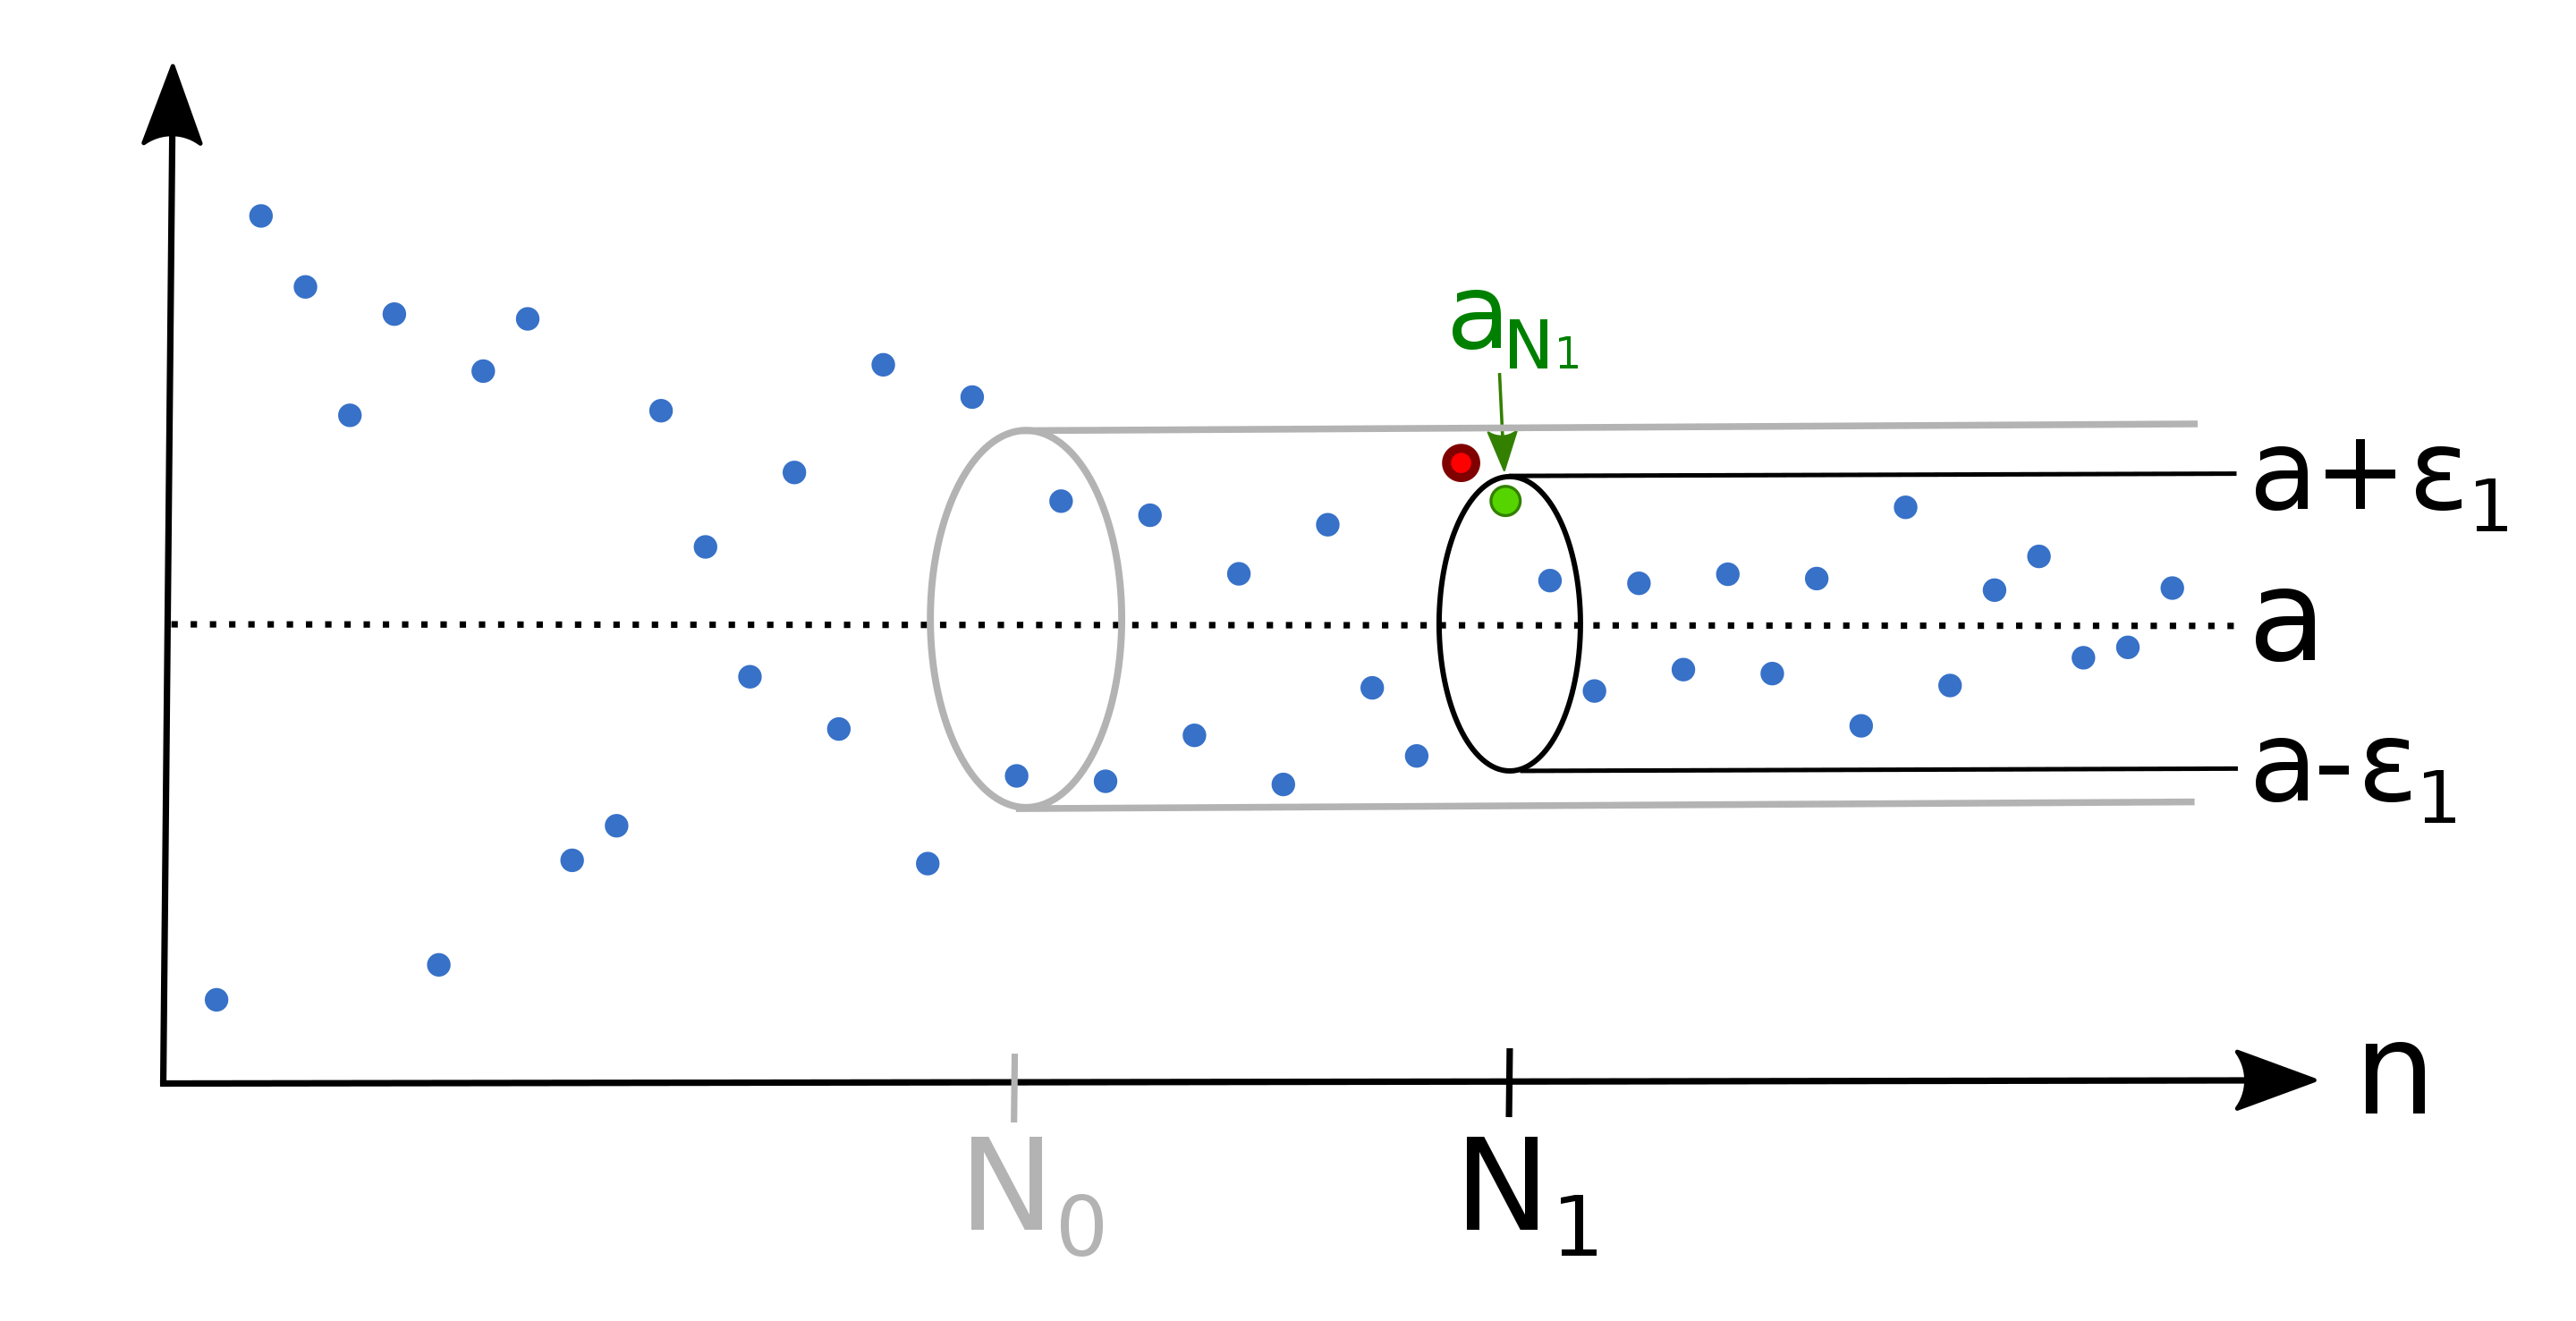
\includegraphics[width=\linewidth]{figures/limit.png}
    \caption{$a$ denotes the limit in this sequence, $N_0$ denotes $N(\epsilon_0)$ for some $\epsilon_0$, and $N_1 = N(\epsilon_1) < N_0$ for some $\epsilon_1 < \epsilon_0$.}
    \label{fig:conv}
\end{figure}
Proving that a sequences converges comes down to providing the $N$ that makes the terms $x_N, x_{N+1}, x_{N+2}, ...$ all be $\epsilon$-close to $x$.
\begin{exm}
    Prove that $(\frac{1}{n})_{n=1}^{\infty}$ converges to 0.
    \label{exm1}
\end{exm}
\begin{proof}
    Take an $\epsilon > 0$. We require that $|x_n - x| < \epsilon$.
    \begin{align*}
        |x_n - x| &= |\frac{1}{n} - 0|\\
        &= \frac{1}{n}\\
        &< \epsilon\\
        \implies n &> \frac{1}{\epsilon}
    \end{align*}
    So, choose $N$ to be any integer with $N > \frac{1}{\epsilon}$, and we will have that $\frac{1}{n} < \epsilon$ for all $n \leq N$. The result is shown.
\end{proof}
\begin{exm}
    Prove that $(e^{-n})_{n=1}^\infty$ converges to 0.
    \label{exm2}
\end{exm}
Before we continue, let us do some sanity checks (which I believe are really important in any math course). Because $e_{-n}$ decays to 0 {\bf faster} than $\frac{1}{n}$, we expect the $N$ that makes $e_{-n} < \epsilon$ (for all $n \geq N$) to be {\bf smaller} than that of $(\frac{1}{n})$. Why? For a fixed precision $\epsilon$, $e_{-n}$ should get $\epsilon$ away from zero at an earlier index of the sequence than $\frac{1}{n}$. Let's check if that is the case.
\begin{proof}
    Take an $\epsilon > 0$. We require that $|x_n - x| < \epsilon$.
    \begin{align*}
        |x_n - x| &= |e^{-n} - 0|\\
        &= e^{-n}\\
        &< \epsilon\\
        \implies n &> \ln \left(\frac{1}{\epsilon}\right)
    \end{align*}
    So, choose $N$ to be any integer with $N > \ln \left(\frac{1}{\epsilon}\right)$, and we will have that $e^{-n} < \epsilon$ for all $n \leq N$. The result is shown.
\end{proof}
This is what we expected. For reference, letting $\epsilon = 10^{-3}$, we have that $\frac{1}{\epsilon} = 1000$, while $\ln \left(\frac{1}{\epsilon}\right) \approx 7$.

\section{January 13, 2020}

While the definition of {\bf convergence} is beautiful in that it explains as aspect of infinity without ever mentioning it, there is a limitation. In order to say that $(x_n)$ converges, we must know its limit. An observation of sequences that converge might help us derive a necessary and sufficient condition for convergence (in $\R$) that does not require knowledge of the limit. Many sequences can be evaluated by computers for example, if the limit is known to exist.
\begin{defi}[Cauchy Sequence]
    A sequence $(x_n)$ is called Cauchy if for all $\epsilon > 0$, there exists an $N$ (dependent on $\epsilon$) such that
    \begin{align*}
        \forall k,l \geq N, \quad |x_k - x_l| < \epsilon 
    \end{align*}
\end{defi}
\begin{exm}
    Prove that $(\frac{1}{n})_{n=1}^\infty$ is Cauchy.
\end{exm}
\begin{exm}
    Prove that $(e^{-n})_{n=1}^\infty$ is Cauchy.
\end{exm}
We would like to approach the following equivalence result.
\begin{thm}
     A sequence in $\R$ converges if, and only if, it is Cauchy.
\end{thm}
\begin{proof}[Proof of forward direction.]
    We start by assuming sequence $(x_n)$ is convergent with limit $x$. Take any $\epsilon > 0$. Choose $N$ to be large enough such that $|x_n - x| < \frac{\epsilon}{2}$ for all $n \geq N$. Then, for $k, l \geq N$:
    \begin{align*}
        |x_k - x_l| = |x_k - x + x - x_l| \leq |x_k - x| + |x - x_k| \leq \frac{\epsilon}{2} + \frac{\epsilon}{2} = \epsilon
    \end{align*}
\end{proof}
\begin{exm}
    Prove that $(\frac{1}{n})_{n=1}^\infty$ is Cauchy.
\end{exm}
\begin{proof}
    Take any $\e > 0$. Choosing $N > \frac{2}{\e}$, and any $k, l \geq N$,
    \begin{align*}
        |x_k - x_l| &= \left|\frac{1}{k} - \frac{1}{l}\right| \leq \frac{1}{n} + \frac{1}{n} = \frac{2}{n} \leq \frac{2\epsilon}{2} = \epsilon
    \end{align*}
\end{proof}
\begin{exc}
    Prove that $(e^{-n})_{n=1}^\infty$ is Cauchy.
\end{exc}
\begin{defi}[Subsequence]
    Let $(x_n)$ be a sequence. Let $(n_k)_{k=1}^{\infty}$ be a sequence such that $n_1 < n_1 < n_3 < ...$ and each $n_k \in \N$. Then the sequence $(x_{n_k})_{k=1}^\infty$ is called a subsequence of $(x_n)$.
\end{defi}
\begin{exc}
    Prove that every subsequence of a convergent sequence converges (to the same limit).
\end{exc}
\begin{defi}[Bounded Sequence]
    A sequence $(x_n)$ in $\R$ is called bounded if $\E M > 0$ such that $|x_n| \leq M$ for all $n \in \N$.
\end{defi}
\begin{defi}[Monotone Sequence]
    A sequence $(x_n)$ in $\R$ is called monotone non-decreasing if $x_1 \leq x_2 \leq x_3 \leq ...$. Similarly, $(x_n)$ is called monotone non-increasing if $x_1 \geq x_2 \geq x_3 \geq ...$. $(x_n)$ is called monotone if it is either monotone non-increasing or monotone non-decreasing.
\end{defi}
\begin{thm}
    Every sequence in $\R$ has a monotone subsequence.
    \label{thm:mono}
\end{thm}
\begin{proof}
    Let $(x_n)$ be a sequence. Let a {\bf peak} of $(x_n)$ be an element $x_m$ such that if $n > m$, then $x_n < x_m$. That is, $x_m$ is greater than every element that comes after it. Consider two cases. 
    \begin{enumerate}
        \item There are infinitely many peaks $x_{m_1}, x_{m_2}, ...$ for $m_1 < m_2 < ...$. Then these peaks form a non-increasing subsequence, as $x_{m_1} \geq x_{m_2} \geq ...$.
        \item There are finitely many peaks. Let $x_M$ be the last peak. Let $m_1 = M + 1$ Then, $x_{m_1}$ is not a peak, and there exists an $m_2 > m_1$ such that $x_{m_1} \leq x_{m_2}$. $x_{m_2}$ is also not a peak. So there exists another $m_3 > m_2$ such that $x_{m_2} \leq x_{m_3}$. This pattern continues (and can be written inductively), to form a monotone non-decreasing sequence.
    \end{enumerate}
\end{proof}
We'll now present a result that you will show for homework.
\begin{thm}
    Every monotone and bounded sequence converges.
    \label{thm:monobound}
\end{thm}
Using the above ideas, we can prove the following.
\begin{thm}[Bolzano-Weirstrass]
    If a sequence is bounded, it has a convergent subsequence.
    \label{thm:bw}
\end{thm}
\begin{proof}
    By Theorem \ref{thm:mono}, we know that any sequence has a monotone subsequence. If the original sequence is bounded, so is every subsequence. Finally, such a subsequence would be monotone and bounded, thus convergent by Theorem \ref{thm:monobound}.
\end{proof}
Finally, using the above results, we are in a place to prove that Cauchy sequences converge in $\R$.
\begin{thm}
    If a sequence in $\R$ is Cauchy, then it converges.
\end{thm}
\begin{proof}
    We will tackle this in three steps. First, we show that the sequence is bounded. Then we show that the sequences has a convergent subsequence. Lastly, we show that the original sequence converges to the same limit as the subsequence. Let the Cauchy sequence be $(x_n)$.
    \begin{enumerate}
        \item Let $N$ be large enough such that for all $k, l \geq N$, we have that $|x_k - x_l| < 1$. This is possible by applying the definition of Cauchy for the particular case of $\e = 1$. Then, we know that for all $n \geq N$,
        \begin{align*}
            |x_N - x_n| < 1 \implies x_N - 1 < x_n < x_N + 1
        \end{align*}
        So the latter part of the sequence (beyond $N$) is bounded by $\max\{|x_N + 1|, |x_N - 1|\}$. Then part of the sequence from $x_1$ to $x_{N-1}$ is finite, meaning that it is bounded by $\max\{|x_1|, ..., |x_{N-1}|\}$. Letting $M = \max\{|x_1|, ..., |x_{N-1}|, |x_N + 1|, |x_N - 1|\}$, the entire sequence is bounded between $-M$ and $M$.
        \item Now that we know that $(x_n)$ is bounded, we can apply Theorem \ref{thm:bw} to say that there is a convergent subsequence $(x_{n_k})_{k=1}^\infty$. Say this subsequence converges to $x$. In the next step, we will show that $(x_n)$ also converges to $x$.
        \item Take any $\epsilon$. Choose $K$ such that for all $k \geq K$, 
        $|x_{n_k} - x| < \frac{\e}{2}$ (we can do so because the subsequence converges). Then, choose $N_1 > n_K$. Next, let $N_2$ be large enough such that $|x_k - x_l| < \frac{\e}{2}$ (we can do so because $(x_n)$ is Cauchy). Let $N = \max\{N_1, N_2\}$, so that both conditions are satisfied for $n \geq N$. For any $n \geq N$, we have
        \begin{align*}
            |x_n - x| = |x_n - x_{n_K} + x_{n_K} - x| \leq |x_n - x_{n_K}| + |x_{n_K} - x| \leq \frac{\e}{2} + \frac{\e}{2} = \e
        \end{align*}
        The first term is bounded because $n \geq N_2$ and the second term is bounded because $n \geq N_1$. By definition, $(x_n)$ converges to $x$.
    \end{enumerate}
\end{proof}

\section{January 15, 2020}

We'll start with a few sequence problems just to review. First note that the following are equivalent for $x_n, x \in \R$ and $\epsilon > 0$.
\begin{align*}
    |x_n - x| \leq \epsilon \iff x - \epsilon \leq x_n \leq x + \epsilon
\end{align*}
\begin{exc}
    Let $(a_n) \rightarrow L$, $(b_n) \rightarrow L$, and $a_n \leq b_n \leq c_n$ for all $n$. Prove that $(b_n) \rightarrow L$. (This is usually referred to as the Squeeze Theorem)
\end{exc}
\begin{exc}
    Let $(x_n)$ be momnotonically non-decreasing and $(y_n)$ be monotonically non-increasing, and $x_n \leq y_n$ for all $n$. Prove that both of these sequences converge (You will have to use a result from last time). 
\end{exc}
\begin{exc}
    Let $C \in \R$ with $|C| < 1$. Prove that $C^n \rightarrow 0$.
\end{exc}
\begin{exc}
    Show that $\frac{n!}{n^n} \leq \frac{1}{n}$. Then, compute the limit of $(x_n)$ with $x_n = \frac{n!}{n^n}$.
\end{exc}
\begin{exc}
    Let $a \neq b$. Discuss the convergence of the sequence $(x_n)$, with
    \begin{align*}
        x_n = \frac{a^n - b^n}{a^n + b^n}
    \end{align*}
\end{exc}
\begin{exc}
    Let $(x_n) \rightarrow L > 0$. Prove that there is an $N$ such that for all $n \geq N$, $x_n > \frac{L}{2}$.
\end{exc}

\begin{exm}
    What is the supremum and infimum of $\{\frac{(-1)^n}{n} : n = 1, 2, 3, ...\}$?
\end{exm}
\begin{exm}
    Let $0 < r < 1$ be fixed. What is the supremum and infimum of $\{(1+\frac{r}{n})^n : n = 1, 2, 3, ...\}$? 
\end{exm}
\begin{exm}
    What is the supremum and infimum of $[0, 10) = \{x: 0 \leq x < 10\}$? 
\end{exm}

We will now move into a subfield called topology, in which we discuss the shape, boundaries, and other properties of sets in space.
\begin{defi}[Open Set]
    A set $A \sse \R$ is called open if for every $x \in A$, there is an $\e > 0$ such that $(x - \e, x + \e) \sse A$.
\end{defi}
This is the type of set that has ``no boundaries". Similar to the limit-type proofs, you must show that for every element of the set, a small interval around that element is still fully contained in the set.
\begin{exm}
    Prove that the interval $(0, 1)$ is open.
\end{exm}
\begin{proof}
    Take any $x \in (0, 1)$. Letting $\e = \min\{x, 1 - x\}$, we are assured that $(x - \e, x + \e) \sse A$.
\end{proof}
Draw a picture of the previous example if it is unclear. Note that by convention, the empty set $\emptyset$ is open. We prove some basic properties about open sets.
\begin{exm}
    Prove that the union of two open sets is open.
\end{exm}
\begin{proof}
    Let $A$ and $B$ be open sets. We want to show that $A \cup B$ is open. Let $x \in A \cup B$. One or both of the following could be true.
    \begin{enumerate}
        \item $x \in A$. Because $A$ is open, there is $\e$ such that $(x - \e, x + \e) \sse A \sse A \cup B$.
        \item $x \in B$. Because $B$ is open, there is $\e$ such that $(x - \e, x + \e) \sse B \sse A \cup B$.
    \end{enumerate}
    This choices of $\e$ are not required to be the same; they are individual cases.
\end{proof}
\begin{exm}
    Prove that the intersection of two open sets is open.
\end{exm}
\begin{proof}
    Let $A$ and $B$ be open sets. We want to show that $A \cap B$ is open. Let $x \in A \cap B$, i.e. $x \in A$ and $x \in B$. We know the following are both true. Because $A$ is open, there is $\e_1$ such that $(x - \e_1, x + \e_1) \sse A$. Because $B$ is open, there is $\e_2$ such that $(x - \e_2, x + \e_2) \sse B$. Letting $\e = \min\{\e_1, \e_2\}$, we can be assured that $(x - \e, x + \e) \sse A$ and $(x - \e, x + \e) \sse B$, meaning that $(x - \e, x + \e) \sse A \cap B$. Thus, $A \cap B$ is open.
\end{proof}

The same proof can show that a union of an arbitrary (possibly infinite) number of open sets is necessarily open. The same is not true of intersections, in that only a finite number of intersections will guarantee an open set. Which part of our proof breaks down for an infinite number of sets?
\begin{exm}
    Provide an example of an infinite number of open sets whose intersection is not open.
\end{exm}
\begin{proof}
    Let $A_n = (-\frac{1}{n}, \frac{1}{n})$. The intersection $A = \bigcap_{n=1}^\infty A_n = \{0\}$. A single point cannot be open, as any interval around that point would spill out of the set.
\end{proof}

Our next definition will be intuitively similar to a point "on the boundary".
\begin{defi}[Accumulation Point]
    $y \in \R$ is called an accumulation point (AP) of set $A$ if for any $\e$, there is an $x \in A$ such that
    \begin{align*}
        x \in (y - \e, y + \e) \text{ and } x \neq y
    \end{align*}
\end{defi}
This means that the point is close enough to the set that for every small interval around the point, there is an element of the set that is nearby and different. The following result establishes an equivalence.
\begin{thm}
    Let $y \in \R$ and $A$ be a set with $y \notin A$. $y$ is an AP of $A$ if and only if there exists a sequence $(x_n) \rightarrow y$ with $x_n \in A$ for all $n$.
    \label{thm:ap}
\end{thm}
\begin{proof}
    First assume that $y$ is an AP. We must construct a sequence (using the elements of $A$), that converges to $y$. To generate element $x_n$ of the sequence, consider the interval $(y - \frac{1}{n}, y + \frac{1}{n})$ about $y$. By definition of an $AP$, this must contain a point in $A$. Call that $x_n$. Now, given any $\e > 0$, the elements $x_n$ with $n > \frac{1}{\e}$ will be $\e$-close to $y$. Thus, this choice of $(x_n)$ clearly converges to $y$
    
    On the other hand, assume that such a sequence exists. By definition of a convergent sequence, we know that for any $\e$, there exists $N$ such that for all $n \geq N$, $|x_n - y| < \e \iff x_n \in (y - \e, y + \e)$ (there are an infinite number of points in this interval, but we only need one). Now we must only be sure that $y \neq x_n$. By assumption $x_n \in A$, while $y \notin A$, so that cannot be equal. The result is shown.
\end{proof}
Not that we did not use the fact that $y \notin A$ for the forward direction of the proof.

\section{January 16, 2020}

Review the definition of open set and accumulation point (AP) from last time. Now we characterize a set that includes its boundaries.
\begin{defi}[Closed Set]
    A set $A \sse \R$ is called closed if it contains all of its accumulation points.
\end{defi}
Simple examples include single points, bracketed intervals $[a, b]$, and the non-negative reals $[0, \infty)$.
\begin{exm}
    Prove that the union of two closed sets is closed.
\end{exm}
\begin{proof}
    Let $A$ and $B$ be closed. We must show that $A \cup B$ is closed. Accordingly, let $y$ be an AP of $A \cup B$. This should imply that it is a member of $A \cup B$. It is sufficient to show that $y$ is an AP of $A$ or an AP of $B$, because if $y$ was an AP of $A$, then it would be in $A$, as $A$ is closed. The same is true for $B$. If $y$ is in either set, then $y \in A \cup B$. We will show this by contrapositive, in that if $y$ is both not an AP of $A$ and not an AP of $B$, then it is not an AP of $A \cup B$. By assumption, we know that
    \begin{enumerate}
        \item $y$ is not an AP of $A$ implies that there exists $\e_1$ such that $(y - \e_1, y + \e_1)$ does not contain any $x \in A$ with $y \neq x$.
        \item $y$ is not an AP of $B$ implies that there exists $\e_2$ such that $(y - \e_2, y + \e_2)$ does not contain any $x \in B$ with $y \neq x$.
    \end{enumerate}
    Letting $\e = \min\{\e_1, \e_2\}$, the interval $(y - \e, y + \e)$ does not contain any $x$ in $A$ or in $B$ with $y \neq x$. Thus, $y$ is not an AP of $A \cup B$ and the result is shown.
\end{proof}
As you saw last time, this argument breaks down in the case an infinite number of sets. Therefore, only a the union of a finite number of closed sets is guaranteed closed.
\begin{exm}
    Give an example of an infinite union of closed sets that is not closed.
\end{exm}
Such an example could look like $A = \bigcup_{n=1}^\infty A_n$, where $A_n = \{\frac{1}{n}\}$. This set is missing $0$, as it is an AP. For homework, you will prove the following.
\begin{exc}
    Prove that the intersection of two closed sets is closed.
\end{exc}
Unfortunately, it is not true that a set that is ``not open" is automatically "closed". We can find sets that are both and neither (see the concluding examples). However, there is a relationship.
\begin{defi}[Set Complement]
    The set complement $A^c$ of set $A$ in $\R$ is defined as $A^c = \{x \in \R: x \notin A\}$.
\end{defi}

\begin{exc}
    Show using Venn diagrams or De Morgan's laws that $(A \cup B)^c = A^c \cap B^c$ and that $(A \cap B)^c = A^c \cup B^c$.
\end{exc}
The establish the following two results.
\begin{thm}
    If $A \sse \R$ is closed, then $A^c$ is open.
\end{thm}
\begin{proof}
    Let $A$ be closed, and let $x$ be any point in $A^c$. We are confident that $x$ is not an AP of $A$, because then it would be contained in $A$, as as $A$ is closed. So it must be true by the (negated) definition of an AP, there is an $\e > 0$ such that $(x - \e, x + \e)$ contains no points of $A$. We rule out the case that the interval contains a point in $A$ that is equal to $x$, as $x \in A^c$. The entire interval $(x - \e, x + \e)$ is thus contained in $A^c$, as all of the points are not in $A$. By definition, $A$ is open.
\end{proof}
\begin{thm}
    If $A \sse \R$ is open, then $A^c$ is closed.
\end{thm}
\begin{proof}
    Let $A$ be open, and let $y$ be an AP of of $A^c$. Assume for the sake of contradiction, that $y \notin A^c$, i.e. $y \in A$. If so, then for all $\e$, $(y - \e, y + \e)$ contains a point in $A^c$, by definition of an AP. But then, no interval about $y \in A$ is fully contained in $A$, as it would always contain a point in $A^c$. Thus, $A$ is not open. This, however, is a contradiction, and our assumption that $y \notin A^c$ is false. Thus, $y \in A^c$, and $A^c$ is hence closed.
\end{proof}
Another way to phrase the two results in one is by saying that ``$A$ is open if and only if $A^c$ is closed" (work this out using contrapositives!). 

\begin{exc}
    Prove that $\R$ and the empty set $\emptyset$ are both open and closed.
\end{exc}
\begin{exc}
    Provide an example of a set that is neither open nor closed.
\end{exc}
\begin{exc}
    Let $A = \{x : x \text{ is rational.}\}$. Is $A$ open, closed, both, or neither?
\end{exc}
\begin{exc}
    Let $A = \{x : x \text{ is irrational.}\}$. Is $A$ open, closed, both, or neither?
\end{exc}
\begin{exc}
    Let $A = \bigcap_{n=1}^\infty [-2, \frac{1}{n})$. Is $A$ open, closed, both, or neither?
\end{exc}

We now approach our final topological term - compactness. There are a few ways to view this concept. We use compactness to describe the sets that have similar properties when deformed continuously (in ways such as stretching, shrinking, etc.). We can also think of it as those sets that have its elements tightly-packed, with no holes, and no escaping the set. Before the definition, we give a characterization that will help you think about what kinds of sets are compact.
\begin{thm}[Heine-Borel]
    A set $A \in \R$ is compact if and only if it is closed and bounded.
    \label{thm:hb}
\end{thm}
While we will only work with this in $\R$ mathematically, it is helpful to visualize this in $\R^2$. See Figure \ref{fig:compact}.
\begin{figure}
    \centering
    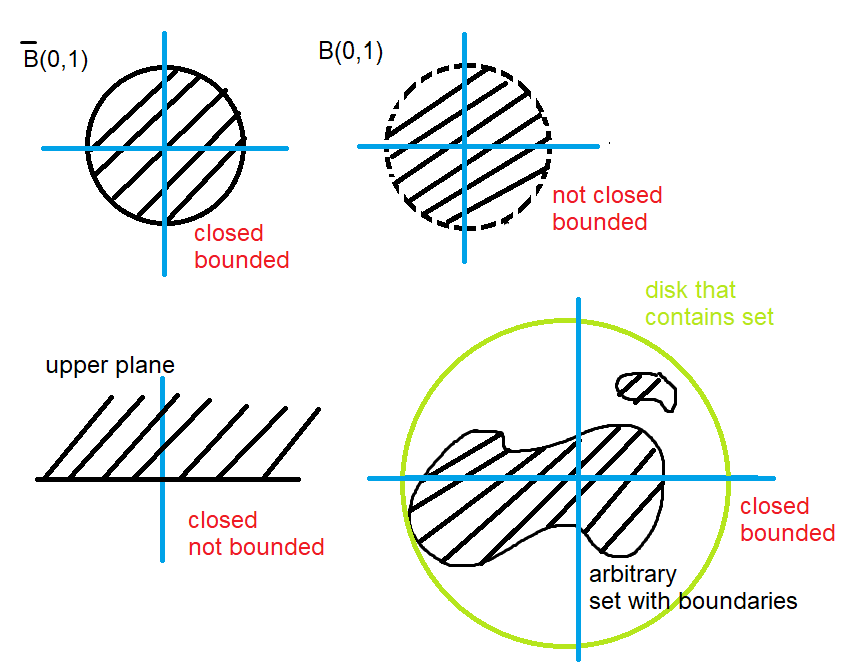
\includegraphics[width=\linewidth]{figures/compact.png}
    \caption{The shaded regions represent elements of the set, with solid and dotted boundaries denoting inclusion and exclusion, respectively. The top-left and bottom-right are compact sets in $\R^2$.}
    \label{fig:compact}
\end{figure}
Now, we look at the definition, which is a little bit more elusive.
\begin{defi}[Compact Set]
    A set $A \in \R$ is compact if for every sequence $(x_n)$ with $x_n \in A \ \forall n$, $(x_n)$ has a subsequence that converges in $A$.
\end{defi}
This can be thought of as all sequences being ``trapped" in $A$, unable to escape to another element even in the limit. We will prove \ref{thm:hb} in pieces.
\begin{exm}
    Prove that a compact set is closed.
\end{exm}
\begin{proof}
    We prove this by contrapositive. Assume set $A$ is not closed. Then, there must exist an AP $y$ of $A$ that lies outside of $A$. By \ref{thm:ap}, we know that there exists a sequence $(x_n)$ with each element in $A$ that converges to $y$. Because $(x_n) \rightarrow y$, any subsequence $(x_{n_k}) \rightarrow y \notin A$. Because we found a sequence in $A$ that does not have a subsequence converging in $A$, $A$ is not compact.
\end{proof}


% BIBLIOGRAPHY AND ACKNOWLEDGEMENTS
% \paragraph{Acknowledgement} Thank you to the students that attended my section this semester. Your feedback has been extremely helpful, and I hope to see you all around in the spring! Good luck on the final!

% \newpage

% \vspace{5mm}
% \bibliography{refs}
% %\bibliographystyle{IEEEtran}
% \bibliographystyle{plainnat}

% \newpage

\end{document}

